\documentclass[crop,tikz]{standalone}
\usepackage{tikz}
\usetikzlibrary{calc}
\usetikzlibrary{positioning}
\begin{document}
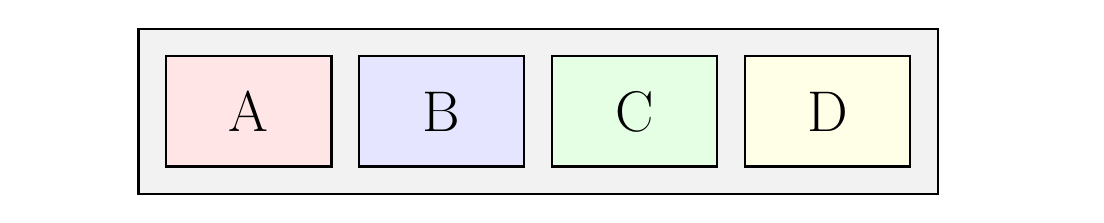
\begin{tikzpicture}[scale=0.07,rotate=0]
		
	%Background
	\draw[draw=white, fill=white] (0,0) rectangle (190,30);	
		
	%Frame
	\draw[thick, draw=black, fill=gray!10] (20,0) rectangle (165,30);

	%Segments
	%A
	\draw[thick, draw=black, fill=red!10] (25,5) rectangle (55,25);
	\node at (40,15) {\huge A};

	%B
	\draw[thick, draw=black, fill=blue!10] (60,5) rectangle (90,25);
	\node at (75,15) {\huge B};
	
	%C
	\draw[thick, draw=black, fill=green!10] (95,5) rectangle (125,25);
	\node at (110,15) {\huge C};
	
	%D
	\draw[thick, draw=black, fill=yellow!10] (130,5) rectangle (160,25);
	\node at (145,15) {\huge D};
	
\end{tikzpicture}
\end{document}